\documentclass[12pt]{article}
\usepackage{graphicx}\usepackage{hyperref}\usepackage{natbib}
\graphicspath{ {../figures/} }

\title{REMARK \LaTeX{} Template}
\author{Econ-ARK Team}
\date{\today}

\bibliographystyle{plainnat}

\begin{document}
\maketitle

\begin{abstract}
The \href{https://github.com/econ-ark/REMARK}{REMARK} infrastructure permits the construction of reproducible scientific computing results, along with associated documentation.
\end{abstract}

\section{Introduction}

\cite{carroll_et_al-proc-scipy-2018} describe plans for the \href{https://econ-ark.org}{Econ-ARK} toolkit, among which is the development of an infrastructure that will allow for the construction of \href{https://econ-ark.org/materials/REMARK}{REMARK} repositories whose aim is to make it easy to construct reproducible scientific computational results.

\section{Other Parts of the Toolkit}

The chief component of the toolkit is the \href{https://github.com/econ-ark/HARK}{HARK} set of tools for solving heterogeneous agent models, particularly of consumption and other financial choices.

Here are some examples produced by the toolkit:

\begin{figure}
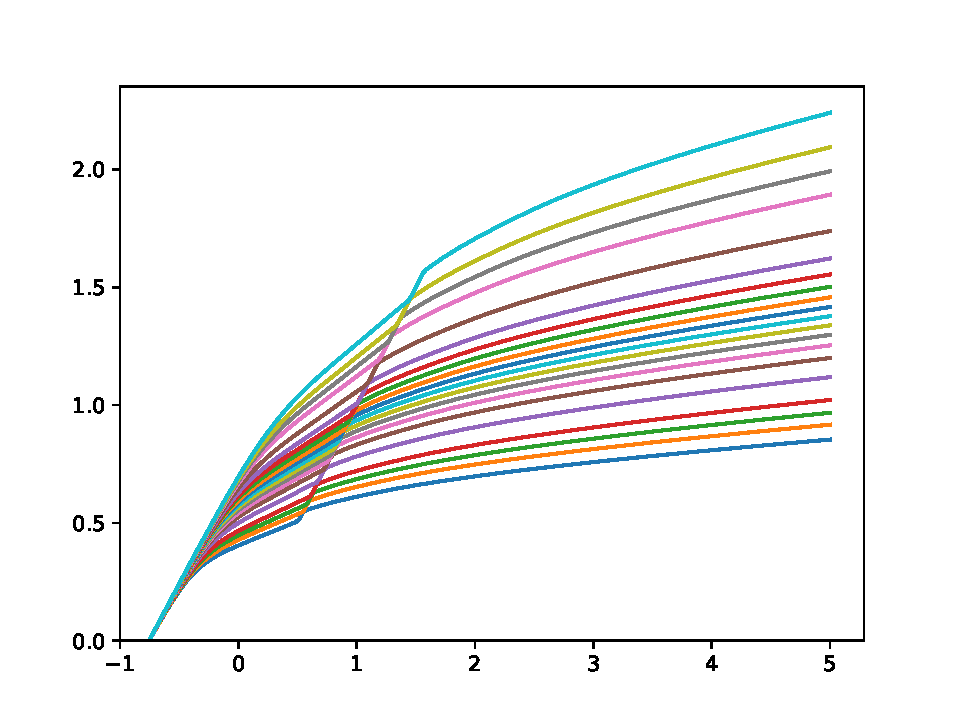
\includegraphics[scale=0.8]{cFunc}
\end{figure}
\begin{figure}
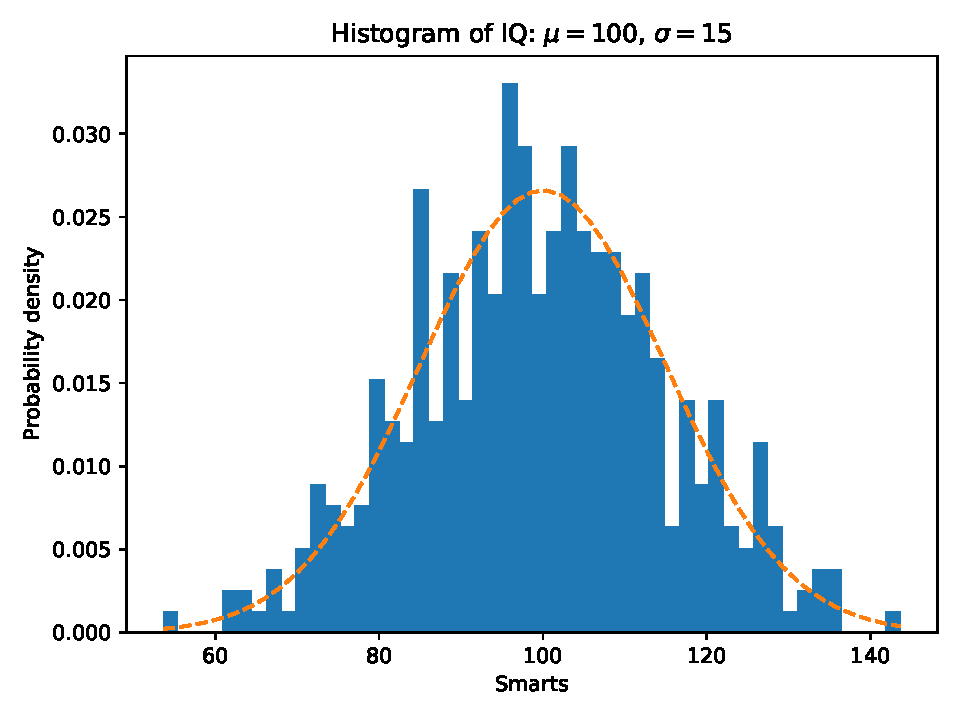
\includegraphics[scale=0.8]{dist}
\end{figure}

\bibliography{./latex/REMARK-starter-example}

\end{document}

% Local Variables:
% eval: (setq TeX-command-list  (assq-delete-all (car (assoc "BibTeX" TeX-command-list)) TeX-command-list))
% eval: (setq TeX-command-list  (assq-delete-all (car (assoc "BibTeX" TeX-command-list)) TeX-command-list))
% eval: (setq TeX-command-list  (assq-delete-all (car (assoc "BibTeX" TeX-command-list)) TeX-command-list))
% eval: (setq TeX-command-list  (assq-delete-all (car (assoc "Biber"  TeX-command-list)) TeX-command-list))
% eval: (add-to-list 'TeX-command-list '("BibTeX" "bibtex latex/%s" TeX-run-BibTeX nil t                                                                              :help "Run BibTeX") t)
% eval: (add-to-list 'TeX-command-list '("BibTeX" "bibtex latex/%s" TeX-run-BibTeX nil (plain-tex-mode latex-mode doctex-mode ams-tex-mode texinfo-mode context-mode) :help "Run BibTeX") t)
% TeX-PDF-mode: t
% TeX-file-line-error: t
% TeX-debug-warnings: t
% LaTeX-command-style: (("" "%(PDF)%(latex) %(file-line-error) %(extraopts) -output-directory=latex %S%(PDFout)"))
% TeX-source-correlate-mode: t
% TeX-parse-self: t
% eval: (cond ((string-equal system-type "darwin") (progn (setq TeX-view-program-list '(("Skim" "/Applications/Skim.app/Contents/SharedSupport/displayline -b -g %n latex/%o %b"))))))
% TeX-parse-all-errors: t
% End:
